\problemname{Deild Goðsagnanna}

Meðlimir Keppnisforritunarfélags Íslands spila Deild Goðsagnanna frekar mikið.
Í Deild Goðsagnanna eru tvö lið, bláa liðið og rauða liðið, og samanstendur hvort þeirra af fimm leikmönnum.
Hver leikmaður fær að velja eina goðsögn til að spila í leiknum áður en leikurinn hefst og engir tveir leikmenn geta valið sömu goðsögnina.

Þessar goðsagnir hafa veikleika og styrkleika og því er mikilvægt að velja réttu goðsögnina sem passa með goðsögnum liðsfélaga og gegn goðsögnum andstæðinga.
Því getur val goðsagnanna skipt miklu máli.
Til að koma í veg fyrir að andstæðingar velji sérstakar goðsagnir má hvort liðið banna val á nokkrum goðsögnum.
Það verður til þess að hvorugt liðið má velja bönnuðu goðsagnirnar.

Ferlið fyrir hvern leik fer fram í eftirfarandi skrefum:
\begin{enumerate}
    \item Bláa liðið bannar eina goðsögn.
    \item Rauða liðið bannar eina goðsögn.
    \item Bláa liðið bannar eina goðsögn.
    \item Rauða liðið bannar eina goðsögn.
    \item Bláa liðið bannar eina goðsögn.
    \item Rauða liðið bannar eina goðsögn.
    \item Bláa liðið velur eina goðsögn.
    \item Rauða liðið velur tvær goðsagnir í röð.
    \item Bláa liðið velur tvær goðsagnir í röð.
    \item Rauða liðið velur eina goðsögn.
    \item Rauða liðið bannar eina goðsögn.
    \item Bláa liðið bannar eina goðsögn.
    \item Rauða liðið bannar eina goðsögn.
    \item Bláa liðið bannar eina goðsögn.
    \item Rauða liðið velur eina goðsögn.
    \item Bláa liðið velur tvær goðsagnir í röð.
    \item Rauða liðið velur eina goðsögn.
\end{enumerate}

Upprunalega voru bara $20$ goðsagnir til að velja um,
\footnote{Í alvörunni voru $17$ goðsagnir upprunalega, en ferlið þurfti einungis $16$ hetjur á þeim tíma.}
en framleiðendur leiksins eru alltaf að bæta við nýjum goðsögnum.
Við segjum að tvö ferli séu mismunandi ef einhver skref eru mismunandi.
Núna er hægt að velja um $n$ goðsagnir, á hve marga mismunandi vegu er hægt velja goðsagnir í liðin?

Athugið að það skiptir einungis máli í hvaða skrefi hver goðsögn er valin eða bönnuð.

Hér að neðan má sjá myndir sem tákna þrjú ferli þar sem lið voru valin.
Bláa liðið er vinstra megin og rauða liðið er hægra megin.
Bannaðar goðsagnir eru í röð frá vinstri til hægri.
Valdar goðsagnir eru í röð frá toppi til botns.

\begin{figure}[h!]
  \centering
    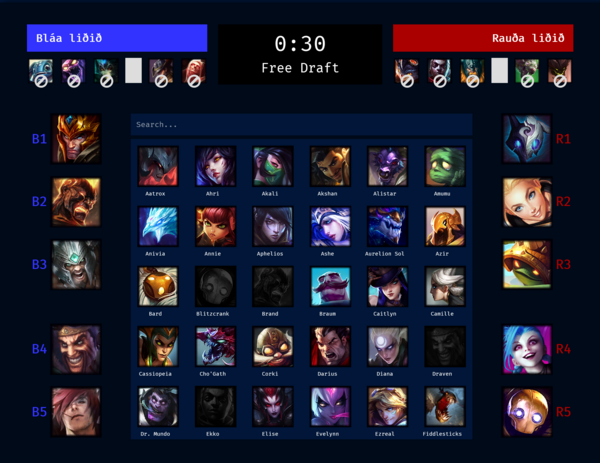
\includegraphics[width=0.8\textwidth]{original_draft.png}
  \caption{Dæmi um ferli þar sem goðsagnir voru bannaðar og valdar.}
\end{figure}

Í ferlinu að ofan gerist eftirfarandi:
\begin{enumerate}
    \item Bláa liðið bannar: Gosi.
    \item Rauða liðið bannar: Gnýr.
    \item Bláa liðið bannar: Örvar.
    \item Rauða liðið bannar: Bergur.
    \item Bláa liðið bannar: Alda.
    \item Rauða liðið bannar: Ólafur.
    \item Bláa liðið velur: Krukkutrukkur, hinn fjórði.
    \item Rauða liðið velur: Ættingi.
    \item Rauða liðið velur: Ljóska.
    \item Bláa liðið velur: Vörumerki.
    \item Bláa liðið velur: Þrándheim.
    \item Rauða liðið velur: Hrútokkur.
    \item Rauða liðið bannar: Kippur.
    \item Bláa liðið bannar: Spjaldimar.
    \item Rauða liðið bannar: Móbergur.
    \item Bláa liðið bannar: Valdimar.
    \item Rauða liðið velur: Strumpur
    \item Bláa liðið velur: Draven.
    \item Bláa liðið velur: Mengi.
    \item Rauða liðið velur: Þrumuþjarki.
\end{enumerate}

\begin{figure}[h!]
  \centering
    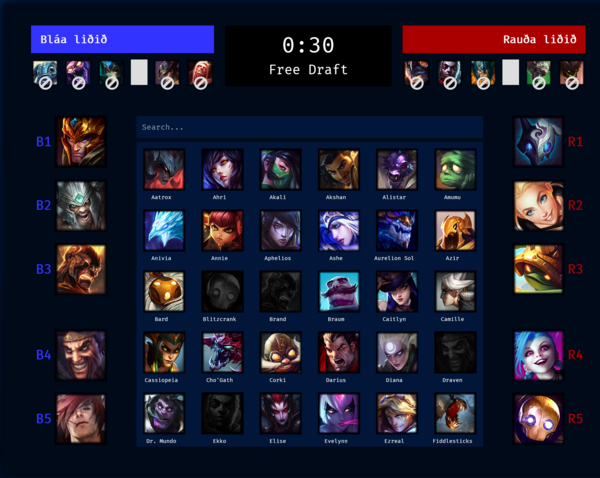
\includegraphics[width=0.8\textwidth]{equivalent_draft.png}
  \caption{Þetta ferli er jafngilt fyrsta ferlinu.}
\end{figure}

Í ferlinu að ofan gerist það sama og í ferlinu á undan, nema bláa liðið velur Þrándheim á undan Vörumerki.
Þetta eru samt sem áður jafngild ferli þar sem þessi tvö völ eiga sér stað í sama skrefi.

\begin{figure}[h!]
  \centering
    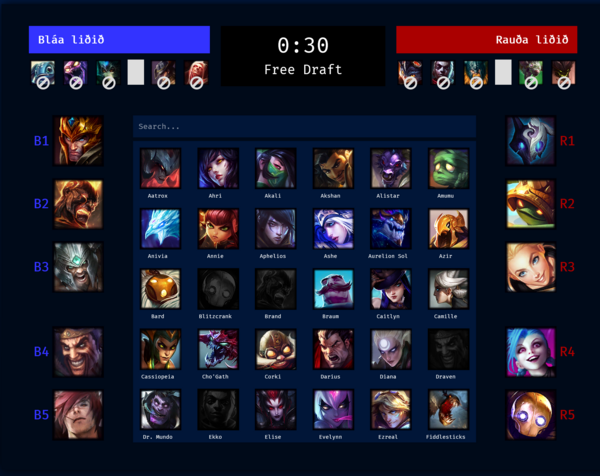
\includegraphics[width=0.8\textwidth]{different_draft.png}
  \caption{Þetta ferli er frábrugðið hinum tveimur ferlunum.}
\end{figure}

Í ferlinu að ofan gerist það sama og í fyrsta ferlinu, nema rauða liðið velur Hrútokkur á undan Ljósku.
Þessi völ eiga sér stað í mismunandi skrefum og því er þetta ferli frábrugðið fyrri tveimur ferlunum.

\section*{Inntak}
Inntak er ein lína með einni heiltölu $n$, fjöldi mismunandi goðsagna sem má velja um í leiknum.

\section*{Úttak}
Segjum að fjöldi leiða til að velja í liðin sé heiltalan $k$.
Athugaðu að $k$ getur verið mjög stór tala.
Því skaltu skrifa út eina línu með einni heiltölu, afganginn við að deila $k$ með $1\,000\,000\,007$.

\section*{Stigagjöf}
\begin{tabular}{|l|l|l|}
\hline
Hópur & Stig & Takmarkanir \\ \hline
1     & 30   & $20 \leq n \leq 21$ \\ \hline
2     & 25   & $20 \leq n \leq 100$ \\ \hline
3     & 20   & $20 \leq n \leq 10^{6}$ \\ \hline
4     & 15   & $20 \leq n \leq 10^{9}$ \\ \hline
5     & 10   & $20 \leq n \leq 10^{18}$ \\ \hline
\end{tabular}
